\section{Golden Ticket}
Windows domains are a very common way to manage network accounts in companies. The servers of this kind of domain are Domain Controllers and the program that handles the domain directory is the Active Directory. The Domain Controller (DC) runs the Key Distribution Center (KDC), which handles Kerberos ticket requests, which are used to authenticate users and allow access to services (for example login).
\linej
The KRBTGT account is the equivalent of a super-administrator account for Kerberos, and is used to encrypt and sign all Kerberos tickets within a domain, so DCs use the account password to decrypt Kerberos tickets for validation. By default this account password never changes and the account name is the same in every domain\cite{stealthbits}.
\linej
\linej
The process to access a service is as follows\cite{tarlogic_theory}\cite{tarlogic_comprehension}:
\begin{enumerate}
	\item The user request a Ticket Granting Ticket (TGT). This ticket is encrypted with the KDC key and is used for request to the KDC one or more Ticket Granting Service (TGS). This request is ciphered with the user hash.
	\item The DC returns the requested TGT is everything is in order.
	\item The user requests the TGS.
	\item The DC returns the requested TGS is everything is in order.
	\item The user sends a request to a computer running a service to make use of it. For this the TGS is sent.
	\item Optionally the Privilege Attribute Certificate (PAC) can be sent to the DC to be verified. The PAC is an structure present in almost every ticket that contains the privileges of the user and it is signed with the KDC key. Nevertheless, the PAC verification consists of checking only its signature, without inspecting if privileges inside of PAC are correct. Furthermore, a client can avoid the inclusion of the PAC inside the ticket by specifying it in KERB-PA-PAC-REQUEST field of ticket request.
	\item Optionally the DC returns the result to the computer that requested it, which should be running the service in question.
	\item Optionally the user receives the response to his request to use the service.
\end{enumerate}

\begin{figure}[H]
	\centering
	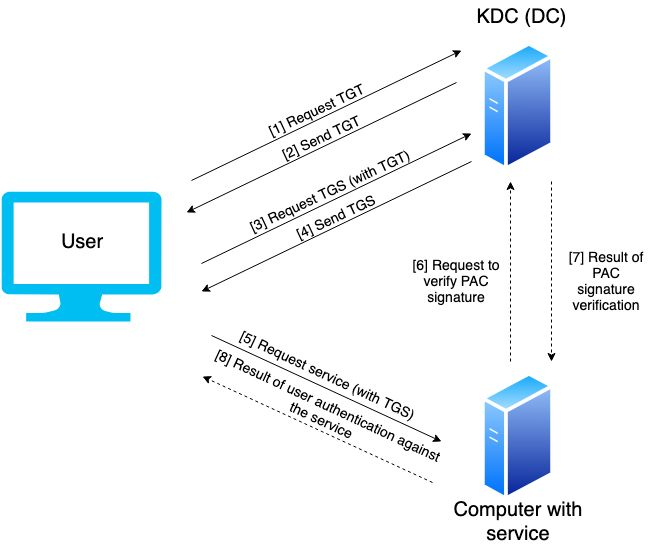
\includegraphics[width=.8\textwidth]{figuras/TGT_TGS_PAC.jpg}
	\caption{Steps for Kerberos authentication}
\end{figure}
\linej
The Golden Ticket attack consists of obtaining the password information of the KRBTGT account to generate a forged TGT, with the desired privileges in the AD, like the AD administrator, this means we can generate TGTs to access every account within the AD. This forged TGT is what we call Golden Ticket.
\linej
The Golden Ticket does not depend at all of the administrator password of the AD, which means that changing this password does not invalidate a Golden Ticket in anyway.
\linej
\linej
Because the attack uses a valid TGT is very hard to detect it is indeed an attack. Once it has been generated the TGT can be used at any time and any amount of times until the time expiration to get a valid TGS from the DC, which is no longer a forgery.
\linej
It follows that this attack should be detected either during the steps needed to create the TGT or by the use of the TGT.
\linej
\linej
The password information of the KRBTGT account can be just the hash of the password, which is stored in memory and can be retrieved with enough local privileges in a DC. To generate the Golden Ticket the attacker also needs the domain name and the SID of the domain to which the KRBTGT account belongs, which are trivial to get\cite{stealthbits}.
\linej
Furthermore once the required data is obtained the Golden Ticket can be generated offline using certain programs, like Mimikatz. This means is impossible to detect the creation of the ticket itself if is not done on a computer in the network, which means only the steps to get the hash of the KRBTGT account can be used to detect the creation of a Golden Ticket.
\linej
\linej
By default Mimikatz sets the forged ticket age to 10 years, which is useful to most attackers because they would need only one attack to compromise the entire network for that time.

\subsection{Exploit methods}
To keep this simple we are only explaining the basics of the techniques used in some of the exploits that can be used for a Golden Ticket attack. Because some of the exploits are similar we number them for easier identification. The scripts in the next exploits were used to understand the different ways to perform Golden Ticket attacks and during the tests to try to detect them. Of course there are more ways to generate a Golden Ticket, and some are much more harder to detect, but there is no time to examine them all. Also it is possible to combine several of the next exploits or change some of their steps.
\linej
For example there is a sever-agent version of Mimikatz called Pypykatz\cite{pypykatz_agent}\cite{pypykatz_server} that is very new and should be a bit harder to detect that the exploits showed here. Unfortunately the student could not make it retrieve the KRBTGT hash.
\linej
\linej
These scripts try to automate as much of the process as possible, which is normally done in an interactive way. This automation helps to ensure that the results are the same each time and reduces the time for each test.

\subsubsection{Exploit 1: Local Mimikatz in DC}
This requires local administrator privileges in the DC and also and an already downloaded version of Mimikatz in the DC, which the attacker can easily get after gaining privileges. If we were to use this example as it is it will probably be detected by the antivirus and Windows Defender, but again they can be disabled by a local administrator and there are techniques to avoid being detected by them.
\linej
\lstinputlisting[style=PS,caption=Script to generate and inject a Golden Ticket in the local DC]{scripts/genticket.ps1}
\linej
The script uses Mimikatz to get the needed data to generate the Golden Ticket, saving it to a file for convenience. Then the data is split in variables, each being a piece for generating the forged ticket. The \textit{exit} parameter is to exit the Mimikatz shell after executing the command.
\linej
After injecting the ticket (with the \textit{/ptt} option) we have administrator privileges in the AD, so we can use any service in the AD in this powershell session, any command we type should be allowed. The id 500 is the normal id for the administrator account in the AD. Without the injection option Mimikatz would store the ticket in a file, which we can inject at any time with Mimikatz. This script can be executed in multiple ways, for example from a powershell interactive terminal run as an administrator.
\linej
\linej
The password hash of the KRBTGT account is retrieved by Mimikatz interacting with the Local Security Authority (LSA) or Local Security Authority Subsystem Service (LSASS), which is run by the lsass.exe process\cite{wikipedia_lsass}\cite{pentestlab}\cite{lsadump_patch_inject}\cite{dump_ways}.
\linej
This process is the Windows service responsible for providing single sign-on functionality, so that users are not required to re-authenticate each time they access resources and it provides access not only to the authenticated user's credentials but every set of credentials used by every open session since the last boot.
\linej
Mimikatz exploits this cache of credentials and reports the results to the user in the various forms employed by LSASS\cite{SANS_mimikatz}.

\subsubsection{Exploit 2: Mimikatz from memory in DC}
This is similar to the previous example but instead of having a downloaded version of Mimikatz (stored in the disk) we download the program directly into the powershell session, so it is not saved to disk.
With slight changes this could work too in a computer that is not a DC if the attacker compromised a workstation a domain admin logged onto\cite{dump_ways}.
\linej
\lstinputlisting[style=PS,caption=Script to run Mimikatz only in memory and inject a Golden Ticket in the local DC]{scripts/genticket.ps1}
\linej
The script downloads a version of Mimikatz from Github and creates a powershell object with its contents, with can be invoked at any time in this shell\cite{powersploit}\cite{powersploit_2}\cite{mimikatz_details}. Then as before it dumps the needed information to generate the Golden Ticket in a file, which is read and parsed to store the interesting parameters into variables.
\linej
I was having trouble trying to automate the last \textit{Invoke-Mimikatz} command to work with the parameters in the variables so as a workaround I write a new file that has the command with those parameters and then I run the file.
\linej
\linej
The clear advantage over the previous one is that it should be harder to detect. This can be easily improved using obfuscation, renaming and not using such an obvious url.

\subsubsection{Exploit 3: Mimikatz with DCSync}
The DCSync is a Mimikatz feature which will try to impersonate a DC and request account password information from the targeted DC. This technique is less noisy as it does not require direct access to a DC (which are often heavily monitored)\cite{dump_ways}\cite{pentestlab}. To run Mimikatz we still need local administrator privileges in the computer.
\linej
\lstinputlisting[style=PS,caption=Script to run Mimikatz with DCSync from a no DC computer in the AD network]{scripts/genticket_dcsync_mimikatz.ps1}
\linej
This follows the same structure as the previous cases, but this time with the dcsync option.
\linej
\linej
The disadvantage in this case is that there needs to be a connection to a running DC that is not being monitored for the requests Mimikatz sends. There are open source tools available for this kind of monitoring\cite{dcsync_monitor}.

\subsubsection{Exploit 4: DCSync with Kiwi}
In this case the access to the no-DC computer in the targeted network is done through Metasploit and its own version of Mimikatz called Kiwi\cite{pentestlab}. We use the Kali virtual machine to execute Metasploit outside the AD, but we could have used a Windows machine running in the AD to do the same.
\linej
We need to know the password of the account we want to access remotely and the targeted computer needs to have a SMB share.
In this case the variable \textit{SMBPass} stores the password, which is \textit{Passw0rd}.
\linej
\lstinputlisting[style=ruby]{scripts/metasploit_p1_kiwi.rc}
This runs a remote process, exploiting the SMB capabilities to run commands to spawn a Meterpreter shell\cite{meterpreter}. This shell has administrator privileges because it started from the administrator share \textit{C\$}, for which we have the administrator account. There is a chance that the \textit{run} command fails to provide a Meterpreter shell at this stage, but trying again always ends working because is just that the session is not getting created even though the exploit is working.
\linej
Now we are in a Meterpreter shell, which we can use to get the exact privileges we need for the next part. This is because even though we have administrator privileges there are different kinds of administrator privileges on Microsoft systems.
\begin{figure}[H]
	\centering
	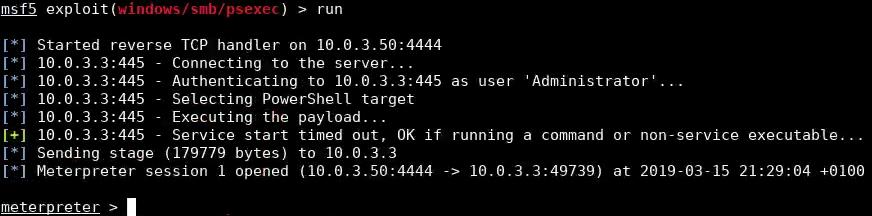
\includegraphics[width=\textwidth]{figuras/meterpreter.png}
	\caption{Meterpreter shell running}
\end{figure}
To do this we look for a session running administrator privileges in the AD. In this case the targeted machine had a powershell session running as administrator, to which we migrate.
\linej
\begin{figure}[H]
	\centering
	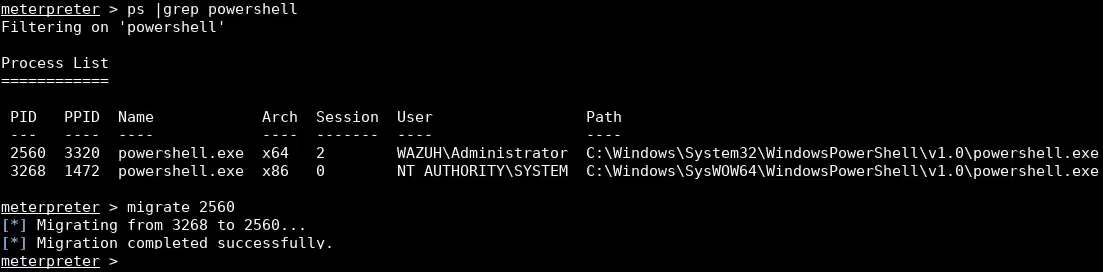
\includegraphics[width=\textwidth]{figuras/migrate.png}
	\caption{Migration to one powershell as local administrator to another as AD administrator}
\end{figure}
Now we are ready to run the real exploit. This loads the Metasploit version of Mimikatz (Kiwi) in the Meterpreter shell, allowing the attacker to use Kiwi commands. The command in this case retrieves the information of the KRBTGT account needed to generate the Golden Ticket, which is used for the last command. In this case the generation of the ticket is not using the data in an automated way, because there was no real need since is the same every time and the time needed to do this with Ruby felt like a waste. In this case the ticket is saved to the \textit{/tmp/golden.tck} file in the Kali machine.
\linej
\lstinputlisting[style=ruby]{scripts/metasploit_p2_kiwi.rc}
\begin{figure}[H]
	\centering
	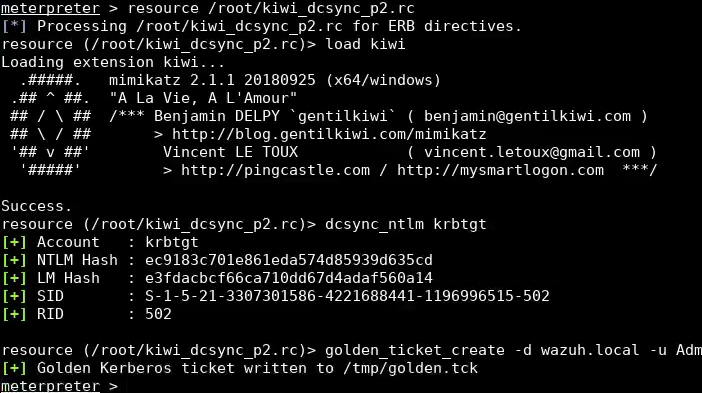
\includegraphics[width=\textwidth]{figuras/kiwi_p2.png}
	\caption{Retrieval of KRBTGT data and generation of the Golden Ticket with DCSync}
\end{figure}
The obvious downside of this method for the attacker is that Metasploit is very widely used and known, therefore there could be security monitoring for it\cite{detect_metasploit_traffic}. But again we are using a technique that does not need to control a DC and does not need to store anything in the disk of the targeted system, making it much harder to detect.
\linej
\linej
Of course there is no real need to use Metasploit to get a remote shell to run Mimikatz. The attacker could use ssh, run remote commands individually with \textit{psexec} or use the Windows Remote Shell. But some of these need to be enabled and they would not be much different of the previous examples.

\subsubsection{Exploit 5: Hashdump with Meterpreter}
Using a reverse tcp exploit the attacker access the targeted DC with a Meterpreter shell. This is similar to the previous case but using the Meterpreter command \textit{hashdump} instead of the DCSync retrieval of Kiwi\cite{pentestlab}. This stills uses Kiwi to generate the Golden Ticket.
\linej
\lstinputlisting[style=ruby]{scripts/metasploit_p1_hashdump.rc}
\linej
Again there is a migration to an administrator account of the AD. In this case another command to get the SID of the network would be needed if we did not know it already, for example a simple \textit{whoami /user} would suffice.
\linej
\lstinputlisting[style=ruby]{scripts/metasploit_p2_hashdump.rc}
\begin{figure}[H]
	\centering
	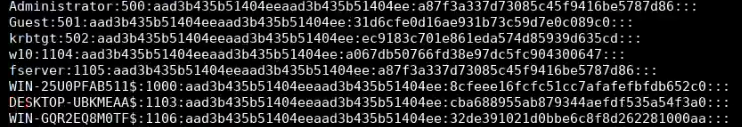
\includegraphics[width=\textwidth]{figuras/hashdump.png}
	\caption{Retrieval of KRBTGT data with hashdump}
\end{figure}
As before it is expected of the DCs to be more monitored. This means that the DCSync version is more interesting to an attacker because it has the same difficulty and beneficts at a lower risk.

\subsubsection{Exploit 6: Retrieval of NTDS.DIT}
Another way to get the desired information is to copy the database of the AD Domain Services (the NTDS.DIT file) and conduct an offline password audit of the domain. This means once we have this data we can use a wide selection of tools to extract or crack the KRBTGT password.
Fortunately for the attacker there are builtin Microsoft commands to accomplish this without the need to use scripts, third-party tools or injection into running processes\cite{ntdsdit_tools}\cite{ntdsutil_cyberis}\cite{dump_ways}\cite{extracting_ntds}\cite{ntds_powershell}.
\linej
\linej
This case was not automated because is simpler than the rest and it was harder to do so because it uses its own type of shell: \textit{ntdsutil}.
The attacker has to open a shell as administrator in a DC and introduce the next input to create the backup:
\begin{lstlisting}[style=PS,frame=none]
ntdsutil
activate instance ntds
ifm
create full C:\Users\Administrator\Downloads\dump_ntds
\end{lstlisting}
\begin{figure}[H]
	\centering
	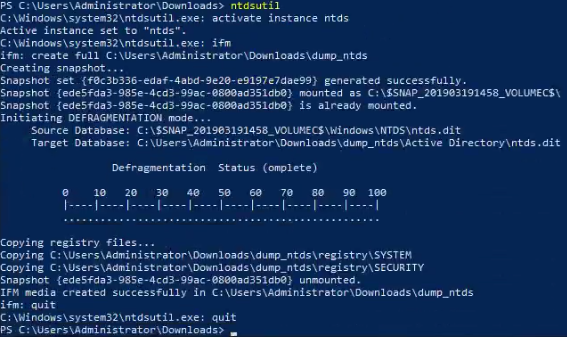
\includegraphics[width=\textwidth]{figuras/ntdsutil.png}
	\caption{Backing up the database of the AD using the ntdsutil shell}
\end{figure}
The new directory contains all necessary files to extract the necessary data to generate a Golden Ticket.
\linej
\linej
There are multiple ways to protect the NTDS.DIT file\cite{protect_NTDS}\cite{hood}:
\begin{itemize}
	\item Monitor or restrict the ntdsutil command.
	\item Backup and disk encryption.
	\item Restrict access to DCs and AD administrators.
	\item Remove the ability to start/stop the Volume Shadow Copy service from ALL users on the system.
	\item Remove the ability to modify the security settings of the Volume Shadow Copy service from all users except for SYSTEM.
\end{itemize}
Of course there is still the task of building the Golden Ticket, for which any of the shown methods would suffice.
\linej
\linej
In our case the easiest measure is to set a rule that is triggered by the existence of a suspicious string related to the \textit{ntdsutil} command:
\begin{lstlisting}[style=xml,numbers=none]
<match>ntds.dit|GLOBALROOT\Device\HarddiskVolumeShadowCopy1\Windows\NTDS</match>
\end{lstlisting}
But of course this is not very efficient and it may be useless.


\subsection{Detection of the attack with Windows events}
In theory we can identify certain attacks with the security events of Windows. There are multiple websites in which this attack has been analyzed and its events identified\cite{events_1}.
Unfortunately the events recorded did not really probe to be the same as the cited sources (probably because we tested on the new Windows Server version, 2019) and they are not enough to be distinguished of the regular activity (which is very bad when we remember we are using a lab environment, without real load). This could probably be improved if these events had more information (particularly those related to Kerberos), but they are very short and generic.
\linej
\linej
Wazuh provides access to Windows events by default, due to the rules and decoders of its ruleset\cite{wazuh_ossec_ruleset}, the user only needs to define rules to specify what and how he wants to monitor.
\linej
We can enable additional logging with the Advanced Audit Policy Configuration. For example for auditing kernel objects, more Kerberos logging, changes in settings or account events. Is worth to mention that this did not probe to be useful for detecting anything in this project, but it was obvious to check it out.
\linej
\linej
The student tried to analyze the security events to find patterns in the previous exploits, by recording all the data received by Wazuh in during their execution. This was done just by looking the current line of the log, executing the exploit and copying the log from there to the end to a new file.
\linej
The obvious problem of this method is that it results in logs with tens to hundreds of lines filled with a not very easy to read format. The workaround used was to parse the logs with custom AWK scripts to remove fields to make the logs more readable and to count each of the events in them.
\linej
\linej
The idea of finding a relationship between certain events and an attack was abandoned because it has already been done\cite{sysmon_event_7_mimikatz} and it was too time consuming and it was not providing any new results. Also it was concerning the amount of noise this method has, even though in a laboratory without real system load.
\linej
\linej
The real useful addition to the Windows builtin events is having Sysmon\cite{sysmon} in each of the monitored Windows computers.
With Sysmon we can have reports of events [1-21] and 255, which in some cases provide very precise and useful information of the system. For example we can configure Sysmon to log data about process with a certain string, like: \textit{powershell}, \textit{Mimikatz}, \textit{.ps1}, \textit{.exe}.
Sysmon can monitor each of the events either by whitelisting or blacklisting by default or both. We can also combine it with rules from Wazuh, using Sysmon to increase the report capabilities and Wazuh to filter them.
\linej
\linej
Also is important to note that Sysmon can be a bit tricky to balance the configuration to get as much suspicious events as possible, while not reporting so much it affects the performance of the network. This is responsibility of the administrators of the network, who also have to tune the configuration to their custom needs.
There are public configs for Sysmon that attempt to provide a good insight of the system while not logging too much data\cite{sysmon_config}.
\linej
With Wazuh we can set rules to filter for suspicious strings, just as many antivirus do, but it can be overcome easily by an attacker. This does not mean that is totally worthless, but that it is not something to focus on.

\subsection{Detection of Mimikatz}
Mimikatz is the tool of choice for this kind of attack for most attackers because it is very effective, easy to use and has multiple ways to be used in different attacks\cite{mimikatz_github}\cite{mimikatz_details}. This is a double edge sword for Mimikatz because it has become one of the programs to look for in antimalware detection programs. In this case we assume these programs have not detected Mimikatz and is up to Wazuh to do it. It is interesting to note that the author of Mimikatz provides ways to detect it, like the YARA rules he maintains\cite{mimikatz_yara_rules} or BusyLights\cite{understanding_powersploit_mimikatz}.
\linej
\linej
Detecting Mimikatz is not a sign of a Golden Ticket attack (unless is clear in the way it is used), but still it is a big and dangerous threat to the system and worth checking out.
\linej
Unfortunately as seen in the exploits before there are multiple ways to execute Mimikatz, in an attempt not to be discovered by known techniques. As we know the techniques to detect or avoid detection evolve with each other over time, so any way we try to detect Mimikatz when is executed in a way that attempts to avoid detection known now may be overcome in the future. This again is the paradox of modern security that affects the other works in this project. The same could be applied to other similar tools.
\linej
\linej
The most basic attempt to detect Mimikatz would be a rule which triggers if there is a match of just one suspicious string related to Mimikatz:
\begin{lstlisting}[style=xml,numbers=none]
<match>pypy|mimi|katz|gentil|kiwi|Benjamin D|/rc4:|/user:Administrator|/ptt|/id:500|krbtgt|lsadump|kerberos::|privilege::</match>
\end{lstlisting}
\linej
Detecting the use of every variant of Mimikatz is virtually impossible, not only because their sheer number due to its popularity but because anyone can compile their own. Therefore the logical way to detect Mimikatz would be to detect the basic step for every version: the interaction with the LSASS and process injection\cite{understanding_powersploit_mimikatz}.
\linej
\linej
Upon a very close study of how Mimikatz interacts with Windows is clear that the execution of certain close events mean the dumping of credentials for a Golden Ticket using Mimikatz. This is called grouping, and even though is a very effective technique it may require a lot of work and in some cases the attack does not produce enough noise or is not easy to tell it apart from the system.
\linej
In this case Sysmon is needed to provide insight on these processes. In particular they can be detected by the event 7 of Sysmon, which identifies the load of images (DLLs)\cite{sysmon}\cite{sysmon_event_7_mimikatz}.
\linej
\linej
For this task is better to configure Sysmon in a whitelisting manner to avoid logging too much. Monitoring these 5 images is enough:
\linej
\lstinputlisting[style=xml,caption=Sysmon monitoring of event 7]{scripts/sysmon_event_7.xml}
\linej
On the manager side the next rules are needed:
\linej
\lstinputlisting[style=xml,caption=Rules for detecting Mimikatz as a group of events]{scripts/rules_event_7_mimikatz.xml}
\linej
The \textit{61609} rule is the parent of these rules because it marks the log as a Sysmon event of type 7. Each of the first five rules matches one of the suspicious DLLs and the last rule identifies the use of all the DLLs in a 10 seconds gap as the dump of credentials by Mimikatz.
\linej
The \textit{frequency} option means that the rule has to be matched that number of times to trigger and is set to 2 because is the minimum value possible. This works because the manager receives 2 different log instances for every of this DLLs, at least in Wazuh 3.9 with Sysmon 9. If that were not the case then this could be accomplished in a similar approximation using 2 rules instead of 5, each with 2 or 3 of the DLLs separated by a logical or sign.

\begin{table}[H]
	\centering
	\begin{tabular}{|l|l|l|}
		\hline
		\rowcolor{gray!30}
		Exploit & Detected & As expected \\ \hline
		Exploit 1: Local Mimikatz in DC& \cellcolor{green!60}Yes& \cellcolor{green!60}Yes\\ \hline
		Exploit 2: Mimikatz from memory in DC& \cellcolor{green!60}Yes& \cellcolor{green!60}Yes\\ \hline
		Exploit 3: Mimikatz with DCSync& \cellcolor{green!60}Yes& \cellcolor{green!60}Yes\\ \hline
		Exploit 4: DCSync with Kiwi& \cellcolor{green!60}Yes& \cellcolor{green!60}Yes\\ \hline
		Exploit 5: Hashdump with Meterpreter& \cellcolor{red!60}No& \cellcolor{green!60}Yes\\ \hline
	\end{tabular}
	\caption{Exploit detection by grouping events}
\end{table}
This method detects the use of Mimikatz in all the ways implemented in this project. The hashdump is not detected because it does not use Mimikatz at all and Kiwi is used only to generate the Golden Ticket, not for data gathering.

\subsection{Detection of the use of the TGT with klist}
We can not always detect when a forged TGT is generated, but the attacker still needs to use it to gain access to the active directory domain with the privileges set in the ticket. The first choice for this task would be to monitor the Kerberos log searching for unusual patterns, but it proved to be more hard than it should, so instead we use scan the cache of Kerberos tickets every few minutes.
\linej
The program to examine the contents of the cache is \textbf{klist}.
\linej
\linej
In order to do this we need to enable the execution of Wazuh's remote commands in the Windows agent and set the properties of the command in the manager in \textit{/var/ossec/etc/shared/default/agent.conf}\cite{wazuh_remote_command}:
\linej
\begin{lstlisting}[style=xml]
<agent_config os="Windows">
	<wodle name="command">
		<disabled>no</disabled>
		<tag>remoteklist</tag>
		<command>powershell C:\\Users\\Public\\Documents\\klist.ps1</command>
		<interval>5m</interval>
		<ignore_output>no</ignore_output>
		<run_on_start>yes</run_on_start>
		<timeout>0</timeout>
		<skip_verification>yes</skip_verification>
	</wodle>
</agent_config>
\end{lstlisting}
\linej
In this case the command is a script to get all the tickets of all the sessions with \textit{klist}, compare the ticket value for the field \textit{TicketExpireHours} with the value of \textit{MaxTicketAge} of the Group Policy (putting the difference in a new field) and parse the output to JSON. Having the output in JSON makes it a bit easier to read from the logs (which is useful to fix any mistake in the script) and removes the need of a decoder in the manager. I got the idea from a very different klist script that only works interactively and reports in plain text\cite{klist_script_idea}.
\linej
Doing this with only powershell ensures it will work in any Windows system without external programs. The downside of this parsing and my limited knowledge of powershell is that the script is a bit bulky and the dependency of the format of the output of klist.
\linej
\lstinputlisting[style=PS,caption=Script to scan and parse to JSON the tickets in the cache]{scripts/klist.ps1}
\lstinputlisting[style=PS,caption=Way to get the MaxTicketAge from the Group Policy]{scripts/report.ps1}
Unfortunately the way to get the data in the last script does not work with remote commands because Windows remote commands only allow certain types of commands. In any case the \textit{MaxTicketAge} value is not normally changed and it requires AD administrator privileges to do it, so due to the time constrains of the project this automation was abandoned. There is also other ways to get the \textit{MaxTicketAge} value, but as mentioned this is not something that we should spend time on.
\linej
\linej
Next there is an example of the difference between the normal output of klist and the string stored in an alert in the manager.

\begin{figure}[H]
	\centering
	\includegraphics[width=.9\textwidth]{figuras/klist_normal.png}
	\caption{Klist listing tickets for a certain session}
\end{figure}
\begin{figure}[H]
	\centering
	\makebox[\textwidth][c]{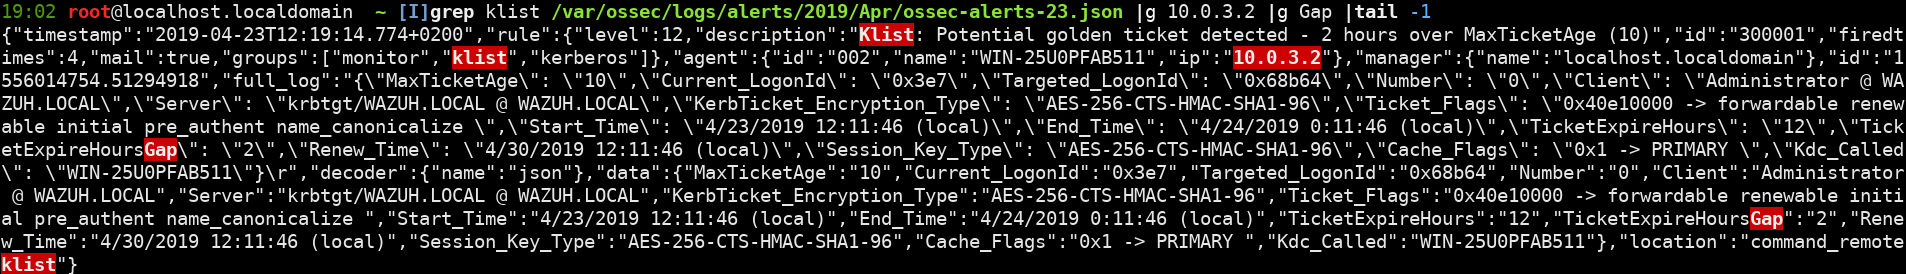
\includegraphics[width=1.2\textwidth]{figuras/klist_alert.png}}
	\caption{Latest alert of the klist monitoring in the manager}
\end{figure}
\linej
The time difference mentioned before is a very easy way to detect a forged ticket. With a simple subtraction in the powershell script only a rule that makes a number comparison in the manager is needed to launch the alert.
\linej
\lstinputlisting[style=xml,caption=Rules to detect a suspicious expiration age from the report of the klist script]{scripts/rule_klist.xml}
\linej
The purpose of the first rule is to identify any log in JSON with \textit{MaxTicketAge} and \textit{TicketExpireHours} fields. The second rule is used to examine the contents of the \textit{TicketExpireHoursGap} field of the logs that the first rule has identified. If the value of the \textit{TicketExpireHoursGap} field starts with a digit different than 0 then it means that \textit{MaxTicketAge} $>$ \textit{TicketExpireHours}, therefore the expiration age is greater that it should, triggering an alert.
Additionally it can only trigger once each 60 seconds, to avoid flooding of alerts.
\linej
\linej
This attack is often used because it may grant the highest privileges in the domain, is hard to detect and is very persistent because it does not care for the password changes in the active directory. That is why is very attractive for domains in which the attacker may decide to come back later, maybe even years later. That means is very unlikely for a forged ticket to not have a very big expiration age, because is one of its most appealing beneficts; but again it would be possible to an attacker to keep generating forged tickets with a valid expiration age forever.
\linej
\linej
The testing of the script was satisfactory, the scripts that inject a TGT were detected and there were no false positives:
\begin{table}[H]
	\centering
	\begin{tabular}{|l|l|l|}
		\hline
		\rowcolor{gray!30}
		Exploit & Detected & As expected \\ \hline
		Exploit 1: Local Mimikatz in DC& \cellcolor{green!60}Yes& \cellcolor{green!60}Yes\\ \hline
		Exploit 2: Mimikatz from memory in DC& \cellcolor{green!60}Yes& \cellcolor{green!60}Yes\\ \hline
		Exploit 3: Mimikatz with DCSync& \cellcolor{green!60}Yes& \cellcolor{green!60}Yes\\ \hline
		Exploit 4: DCSync with Kiwi& \cellcolor{red!60}No& \cellcolor{green!60}Yes\\ \hline
		Exploit 5: Hashdump with Meterpreter& \cellcolor{red!60}No& \cellcolor{green!60}Yes\\ \hline
	\end{tabular}
	\caption{Exploit detection by the klist script}
\end{table}
Of course if we chose to store the ticket in a file we could inject it in other moment or computer, but then it could be detected by this method.
\linej
\linej
Additionally we could monitor looking for unusual usernames, but is not something that is bound to happen, because in most cases the attacker wants the administrator account.

\subsection{Mitigation}
These exploits take advantage of the inherent weaknesses of Kerberos, so there is no way to prevent them. Nevertheless, Microsoft provides a publicly available guide explaining how to mitigate this kind of attacks\cite{microsoft_mitigation}.
The easiest way to mitigate this attack is to change the password of the KRBTGT account to invalidate any existing Golden Ticket, which has to be done twice (make sure the domain converges before doing the second password change\cite{hood}), but it also invalidates existing proper TGTs.
\linej
The recommendation from Microsoft is to regularly reset the password, which can be done with their official script\cite{tarlogic_comprehension}\cite{adsecurity_483}\cite{reset_script}. This could be also triggered by alerts that we are confident detect Golden Tickets, but as mentioned this could affect other functionality and so the decision is for the network administrators to make. Any TGT that is not valid produces an error in a TGS request, which can be used for exposing an attacker\cite{scom_GT}.
\linej
\linej
Also we always can take measures like:
\begin{itemize}
	\item Have administrative passwords longer than 25 characters to avoid brute force cracking and make them unique for each system.
	\item Enforce a least privilege model.
	\item Minimize the quantity of administrative accounts.
	\item Isolate DCs: Use DCs only as servers, never work stations of any kind.
	\item Isolate administrator accounts: Use administrator accounts only for administrator duties.
	\item Isolate AD accounts: Create tiered groups with very granular permissions on the domain and create Access Control List permissions on the Organization Units of the AD\cite{AD_tier}.
	\item Use Read Only Domain Controllers (RODCs): keep Read Write DCs segregated using network segregation and AD sites to force users to logon to RODCs, making breach detection easier. RODCs don't have any real user hashes (nor the hash of the KRBTGT account)\cite{reset_RODC}\cite{hood}.
	\item Use honeypots: With populated the LSASS cache with false credentials\cite{SANS_mimikatz}\cite{honeyhashes} or with decoy AD objects\cite{decoy_AD}. Then we monitor the logs for attempts to use them. This can lead to detect attackers or to find vulnerabilities in the network.
	\item Disable storage of clear text passwords in LSASS memory to limit the information provided by Mimikatz\cite{SANS_mimikatz}.
	\item Run LSASS in protected mode (from Windows 8.1): calls to LSASS are only allowed by other protected-mode processes (Microsoft, 2014, Configuring Additional LSA Protection)\cite{SANS_mimikatz}\cite{understanding_powersploit_mimikatz}.
	\item Use choke points: Create a choke point for access to your DCs, adding another layer of protection. Create a Terminal Server that can only talk to the DCs. Configure the DCs to only accept administrative connections from that Terminal Server\cite{choke}.
\end{itemize}
\linej
We could go on with more detail and increasing the mitigation\cite{AD_defense}, but is not the objective of this project.

\subsection{Conclusion}
We have seen how the data to generate Golden Tickets can be obtained in different ways and the difficulties for both the attacker and the defender roles.
\linej
\linej
Relying on the klist detection means there is no real need to detect each of the different ways to generate the Golden Ticket because it may be impossible depending on the circumstances and more importantly the attacker still needs to present it to a DC to get the TGS to get any benefit from it.
\linej
Detecting certain Sysmon events in a close time gap can guarantee the detection of Mimikatz dumping the needed credentials to generate a Golden Ticket, therefore detecting one of the most used ways to gather this data. Detecting certain strings for running commands, reads and accesses are a worthy way to detect the creation of a Golden Ticket, without spending much resources.
\linej
These are good examples of how detecting common steps to multiple exploits is one of the strong points of an HIDS.
\linej
\linej
Another way of detection is to use YARA to look for certain patterns in memory, just like we can search for strings in the events. In the case of events the data comes from the program, which is easy to modify with multiple techniques like substitution or obfuscation. The patterns in memory are much more harder to change because it involves changing the program logic. That means most attackers would just take the risk to be detected by this kind of technique.
\linej
YARA is very interesting for this kind of project, but it belongs to the Virustotal pack of malware detection tools and so it could be used with Wazuh with a Virustotal API key. The free version only allows a few queries and we didn't consider the option of getting a premium key because there has been for months an open issue in the Github page of Wazuh for integrating it with YARA (as other IDSs have done before), which has recently evolved to an issue to integrate YARA into Wazuh as a module\cite{yara_module}.
%Unfortunately this was not done before this part of the project as completed, so there was no time left to investigate more on it.
%TODO revisar estado issue en el futuro
